% arara: pdflatex: { shell: true }
% arara: xelatex: { synctex: 1, shell: yes }
% arara: lualatex: { shell: true, interaction: nonstopmode }
\documentclass{article}	
\usepackage[a4paper, margin=1in]{geometry}
\usepackage{minted}
\usemintedstyle{manni} % Optional: Set a code style (vs is just an example)
\usepackage{hyperref}
\usepackage{graphicx}
\usepackage{pdfpages}
\usepackage[labelformat=empty]{caption}

\title{Record}
\author{Name}
\date{2023-12-28}

\begin{document}

\includepdf[pages={1}]{./Assets/bob2.pdf}
\newpage
\tableofcontents
\newpage


\section{Simple Html Page}
\subsection{Aim}
\begin{itemize}
	\item Design a webpage for your department.
	\item Utilize paragraphs and lists.
	\item Create links of the words Wifi and LAN to their respective wikipedia pages
	\item Insert an image that redirects to the college website
	\item Change the background color and create a link at the bottom to return to the top
\end{itemize}

\subsection{Code}
\inputminted[frame=lines, breaklines, breakanywhere, numberblanklines=false]{html}{./prog_1/index.html}

\newpage
\subsection{Output}
\begin{figure}[h!]
	\centering
	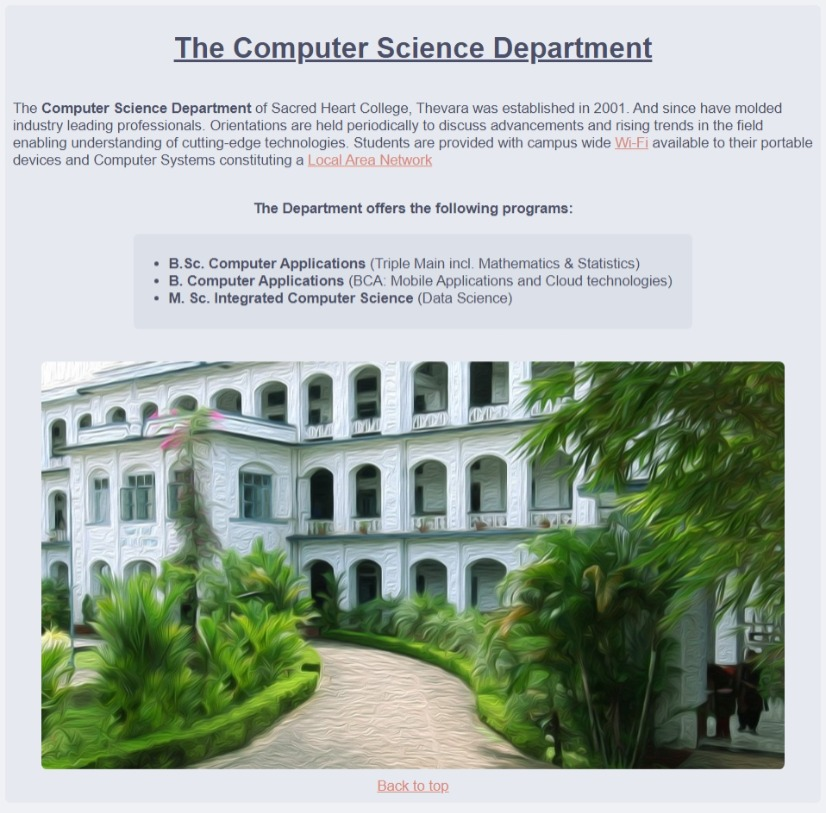
\includegraphics[width=1\textwidth]{./Assets/p0101.jpeg}
\end{figure}
\newpage

\section{Time Table}
\subsection{Aim}
\begin{itemize}
	\item Design the class time table in HTML using table tag
\end{itemize}

\subsection{Code}
\inputminted[frame=lines, breaklines, breakanywhere, numberblanklines=false]{html}{./prog_2/index.html}

\newpage
\subsection{Output}
\begin{figure}[h!]
	\centering
	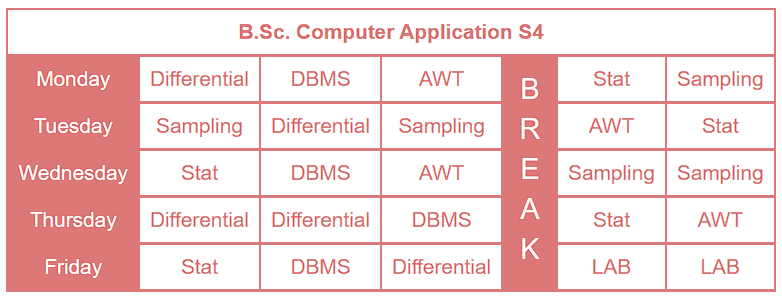
\includegraphics[width=0.8\textwidth]{./Assets/p0201.png}
\end{figure}
\newpage

\section{CSS}
\subsection{Aim}
\begin{itemize}
	\item utlize inline css for appending styles to html elements
	\item utilize an external css stylesheet
\end{itemize}

\subsection{Code}
\inputminted[frame=lines, breaklines, breakanywhere, numberblanklines=false]{html}{./prog_3/index.html}
external stylesheet
\inputminted[frame=lines, breaklines, breakanywhere, numberblanklines=false]{css}{./prog_3/styles.css}

\subsection{Output}
\begin{figure}[h!]
	\centering
	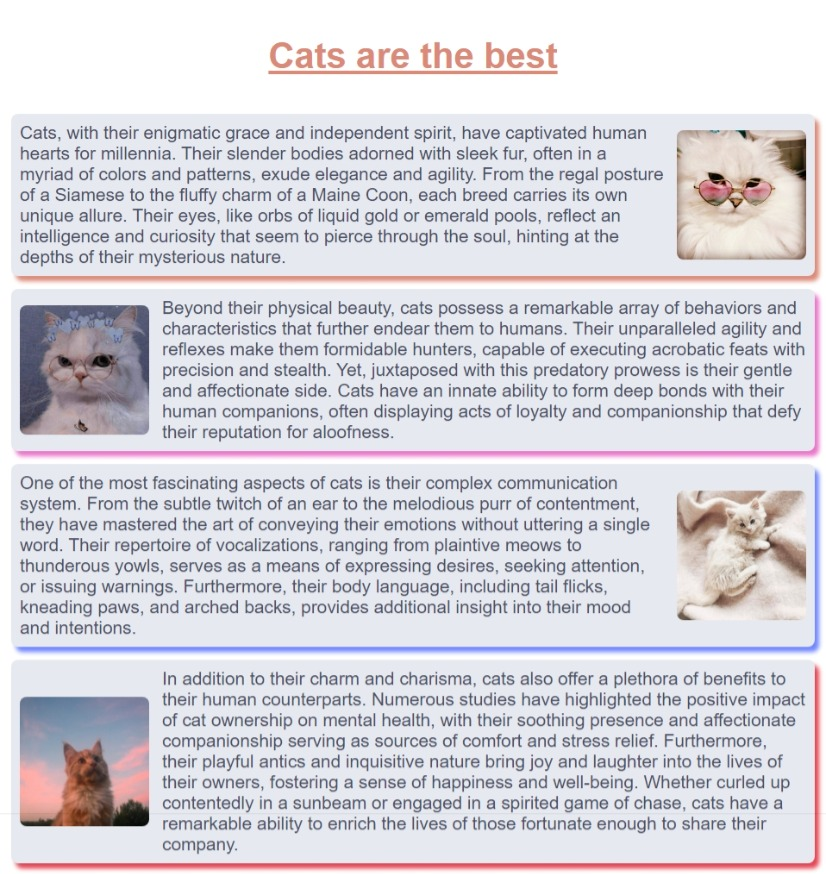
\includegraphics[width=1.0\textwidth]{./assets/p03.jpeg}
\end{figure}
\newpage

\section{Form}
\subsection{aim}
\begin{itemize}
	\item Create a simple form
	\item with fields name age address etc.
	\item include radio buttons checkboxes and a password field
\end{itemize}

\subsection{Code}
\inputminted[frame=lines, breaklines, breakanywhere, numberblanklines=false]{html}{./prog_4/index.html}

\newpage
\subsection{Output}
\begin{figure}[h!]
	\centering
	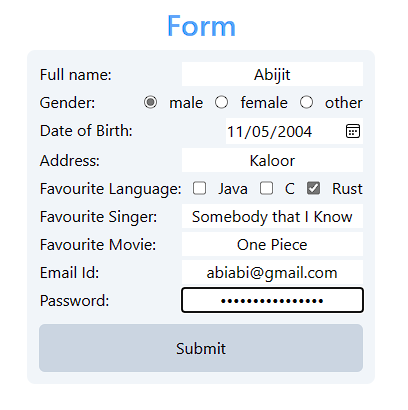
\includegraphics[width=0.4\textwidth]{./Assets/p04.png}
\end{figure}
\newpage

\section{Semester Re-registration Webpage}
\subsection{Aim}
\begin{itemize}
	\item Design a form with the following entries
	\item Enrolment No.
	\item Regional Centre Code (Drop-down)
	\item Study Centre Code (Drop-down)
	\item Semester (Drop-down)
	\item Email Id
\end{itemize}

\subsection{Code}
\inputminted[frame=lines, breaklines, breakanywhere, numberblanklines=false]{html}{./prog_5/index.html}

\subsection{Output}
\begin{figure}[h!]
	\centering
	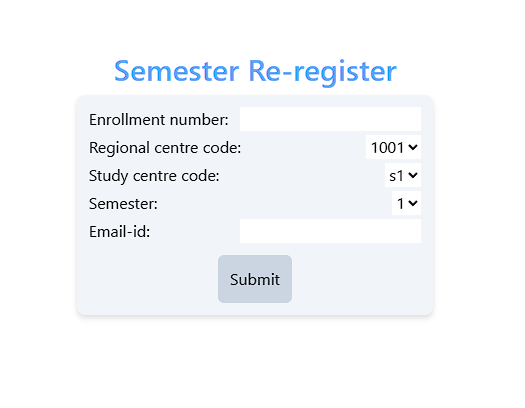
\includegraphics[width=0.6\textwidth]{./Assets/p05.png}
\end{figure}
\newpage

\section{Profit or Loss}
\subsection{Aim}
\begin{itemize}
	\item Write a JavaScript solution for the following
	\item Accept the cost price and selling price with a button
	\item Create a button to calculate the loss or profit and display it
\end{itemize}

\subsection{Code}
\inputminted[frame=lines, breaklines, breakanywhere, numberblanklines=false]{html}{./prog_6/index.html}

\subsection{Output}
\begin{figure}[h!]
	\centering
	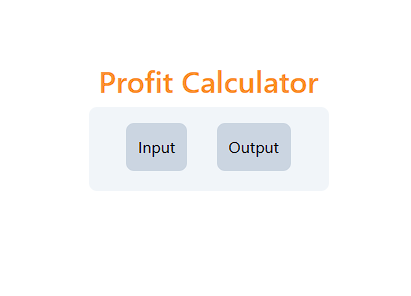
\includegraphics[width=0.5\textwidth]{./Assets/p0601.png}
	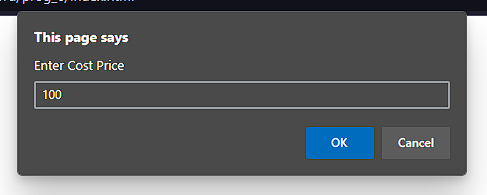
\includegraphics[width=0.5\textwidth]{./Assets/p0602.png}
	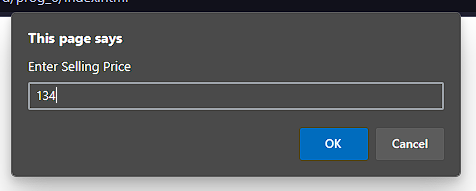
\includegraphics[width=0.5\textwidth]{./Assets/p0603.png}
	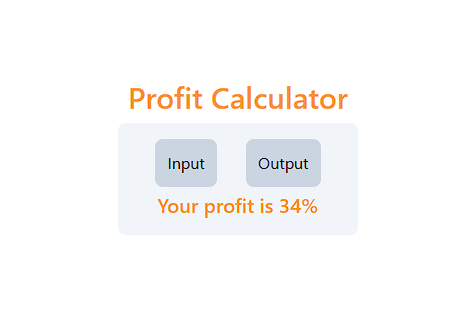
\includegraphics[width=0.6\textwidth]{./Assets/p0604.png}
\end{figure}
\newpage

\section{Electrical Connection Form}
\subsection{Aim}
\begin{itemize}
	\item Create a form with the following fields
	\item Permanent or temporary connection (radio button)
	\item Government or Private house (radio button)
	\item Name and Email
\end{itemize}

\subsection{Code}
\inputminted[frame=lines, breaklines, breakanywhere, numberblanklines=false]{html}{./prog_7/index.html}

\subsection{Output}
\begin{figure}[h!]
	\centering
	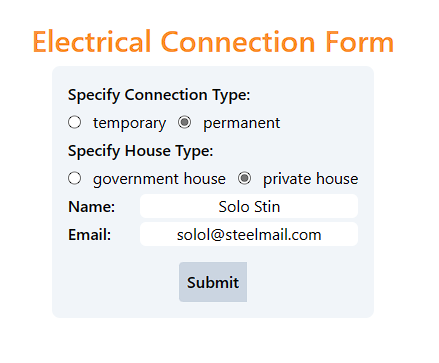
\includegraphics[width=0.6\textwidth]{./Assets/p07.png}
\end{figure}
\newpage

\section{Word Search}
\subsection{Aim}
\begin{itemize}
	\item Write a JavaScript Program to search for a word in a sentence
	\item the search should be performed when a appropriate button is clicked
\end{itemize}

\subsection{Code}
\inputminted[frame=lines, breaklines, breakanywhere, numberblanklines=false]{html}{./prog_8/index.html}

\newpage
\subsection{Output}
\begin{figure}[h!]
	\centering
	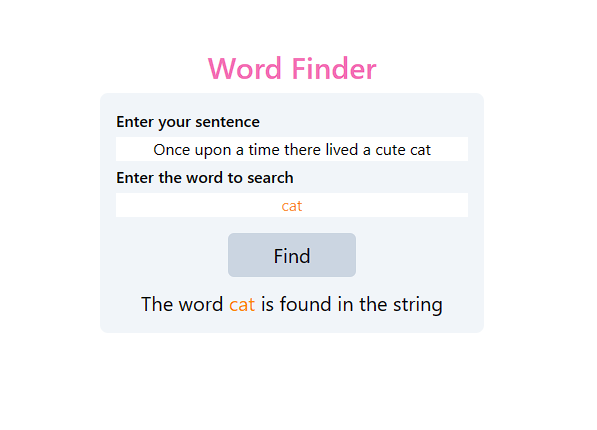
\includegraphics[width=0.8\textwidth]{./Assets/p0801.png}
	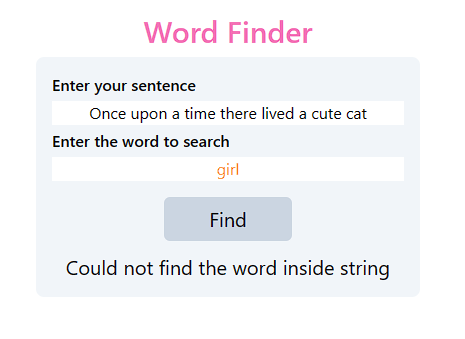
\includegraphics[width=0.6\textwidth]{./Assets/p0802.png}
\end{figure}
\newpage

\section{Prime and Armstrong}
\subsection{Aim}
\begin{itemize}
	\item Write a program to determine whether a number is Armstrong or Prime
\end{itemize}

\subsection{Code}
\inputminted[frame=lines, breaklines, breakanywhere, numberblanklines=false]{html}{./prog_9/index.html}

\subsection{Output}
\begin{figure}[h!]
	\centering
	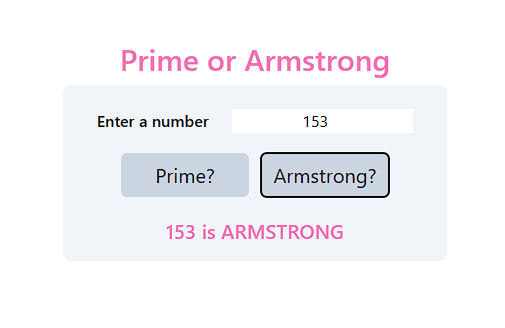
\includegraphics[width=0.6\textwidth]{./Assets/p0901.png}
	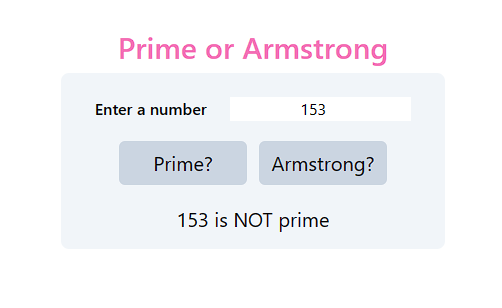
\includegraphics[width=0.6\textwidth]{./Assets/p0902.png}
\end{figure}
\newpage

\section{Fibonacci Series}
\subsection{Aim}
\begin{itemize}
	\item Write a program to display the first n terms of the Fibonacci series
\end{itemize}

\subsection{Code}
\inputminted[frame=lines, breaklines, breakanywhere, numberblanklines=false]{html}{./prog_10/index.html}

\subsection{Output}
\begin{figure}[h!]
	\centering
	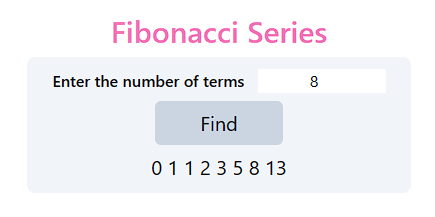
\includegraphics[width=0.4\textwidth]{./Assets/p10.png}
\end{figure}
\newpage

\section{University Login}
\subsection{Aim}
\begin{itemize}
	\item Create a login page
	\item with fields name and enrollment number
	\item After submitting information, redirect to a welcome page
\end{itemize}

\subsection{Code}
index.html
\inputminted[frame=lines, breaklines, breakanywhere, numberblanklines=false]{html}{./prog_11/index.html}
\newpage
login.html
\inputminted[frame=lines, breaklines, breakanywhere, numberblanklines=false]{html}{./prog_11/login.html}

\subsection{Output}
\begin{figure}[h!]
	\centering
	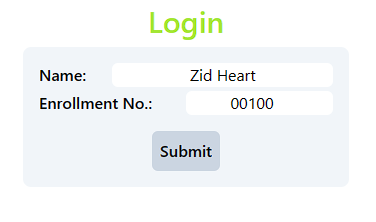
\includegraphics[width=0.4\textwidth]{./Assets/p1101.png}
	
\includegraphics[width=0.8\textwidth]{./Assets/p1102.png}
\end{figure}
\newpage

\section{First Vowel}
\subsection{Aim}
\begin{itemize}
	\item Write a JavaScript program to find the first vowel in a string
\end{itemize}

\subsection{Code}
\inputminted[frame=lines, breaklines, breakanywhere, numberblanklines=false]{html}{./prog_12/index.html}

\subsection{Output}
\begin{figure}[h!]
	\centering
	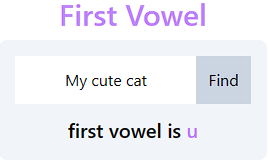
\includegraphics[width=0.25\textwidth]{./Assets/p12.png}
\end{figure}
\newpage

\section{Basic Calculator}
\subsection{Aim}
\begin{itemize}
	\item Write a JavaScript program implementing a Simple Calculator
\end{itemize}

\subsection{Code}
\inputminted[frame=lines, breaklines, breakanywhere, numberblanklines=false]{html}{./prog_13/index.html}

\newpage
\subsection{Output}
\begin{figure}[h!]
	\centering
	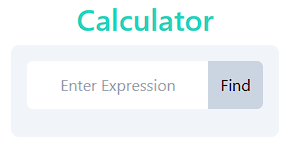
\includegraphics[width=0.3\textwidth]{./Assets/p1301.png}
	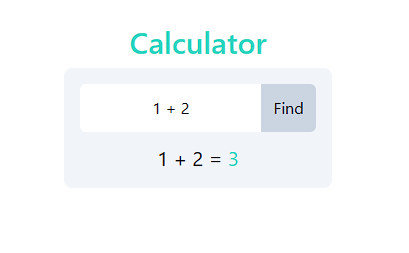
\includegraphics[width=0.5\textwidth]{./Assets/p1302.png}
	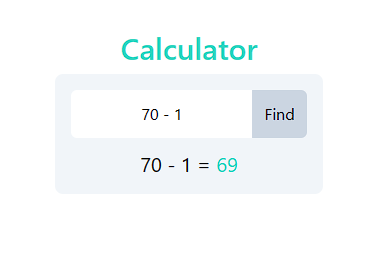
\includegraphics[width=0.5\textwidth]{./Assets/p1303.png}
	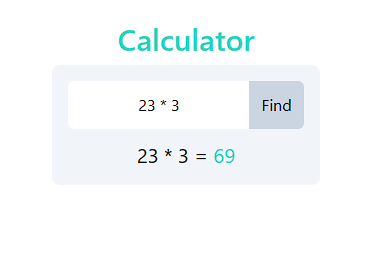
\includegraphics[width=0.5\textwidth]{./Assets/p1304.png}
	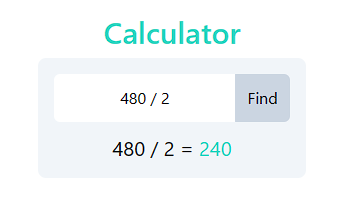
\includegraphics[width=0.5\textwidth]{./Assets/p1305.png}
\end{figure}
\newpage

\section{Company Profile Form}
\subsection{Aim}
\begin{itemize}
	\item Create a form for entering A company Profile
	\item The form should have an update button
	\item update button should update the profile
\end{itemize}

\subsection{Code}
\inputminted[frame=lines, breaklines, breakanywhere, numberblanklines=false]{html}{./prog_14/index.html}

\subsection{Output}
\begin{figure}[h!]
	\centering
	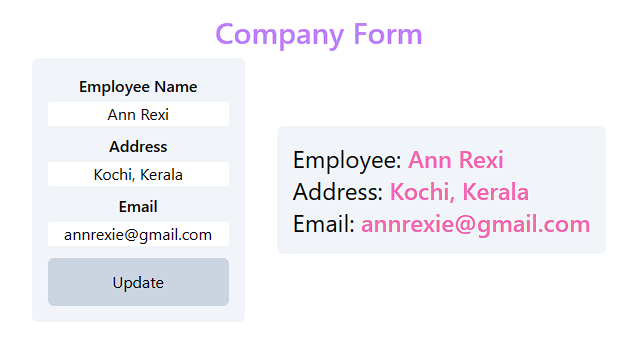
\includegraphics[width=0.8\textwidth]{./Assets/p1401.png}
	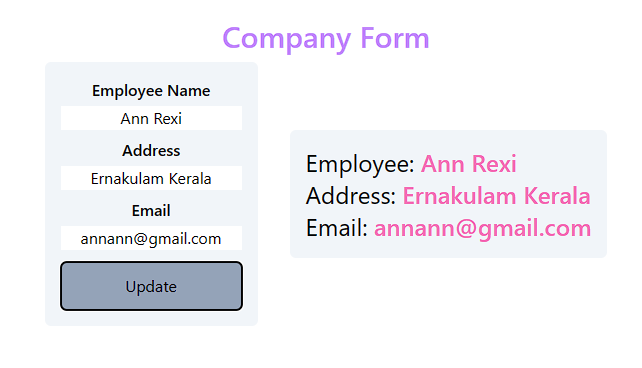
\includegraphics[width=0.8\textwidth]{./Assets/p1402.png}
\end{figure}
\newpage

\section{Random Number}
\subsection{Aim}
\begin{itemize}
  \item Write a JavaScript program to perform the following
	\item validation checks on text and email fields of a form
	\item Generate a random number when a Button is clicked
\end{itemize}

\subsection{Code}
\inputminted[frame=lines, breaklines, breakanywhere, numberblanklines=false]{html}{./prog_15/index.html}

\subsection{Output}
\begin{figure}[h!]
	\centering
	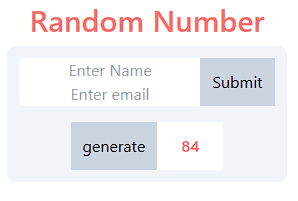
\includegraphics[width=0.4\textwidth]{./Assets/p1501.png}
	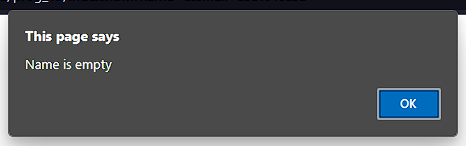
\includegraphics[width=0.4\textwidth]{./Assets/p1502.png}
	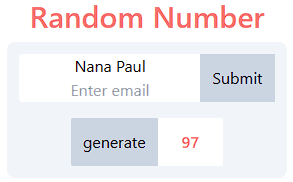
\includegraphics[width=0.4\textwidth]{./Assets/p1503.png}
	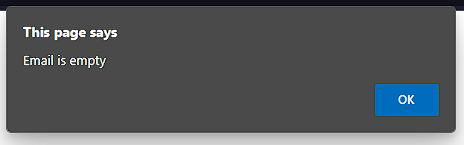
\includegraphics[width=0.4\textwidth]{./Assets/p1504.png}
	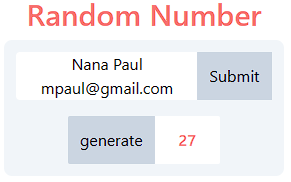
\includegraphics[width=0.4\textwidth]{./Assets/p1505.png}
	
\includegraphics[width=0.4\textwidth]{./Assets/p1506.png}
\end{figure}
\newpage

\section{Company Login Page}
\subsection{Aim}
\begin{itemize}
  \item Design a login page of a  company
  \item with feilds name and password
  \item redirect to the company homepage after clicking login
  \item the homepage must display details of the company
\end{itemize}

\subsection{Code}
index.html
\inputminted[frame=lines, breaklines, breakanywhere, numberblanklines=false]{html}{./prog_16/index.html}
webpage.html
\inputminted[frame=lines, breaklines, numberblanklines=false]{html}{./prog_16/webpage.html}

\newpage
\subsection{Output}
\begin{figure}[h!]
	\centering
	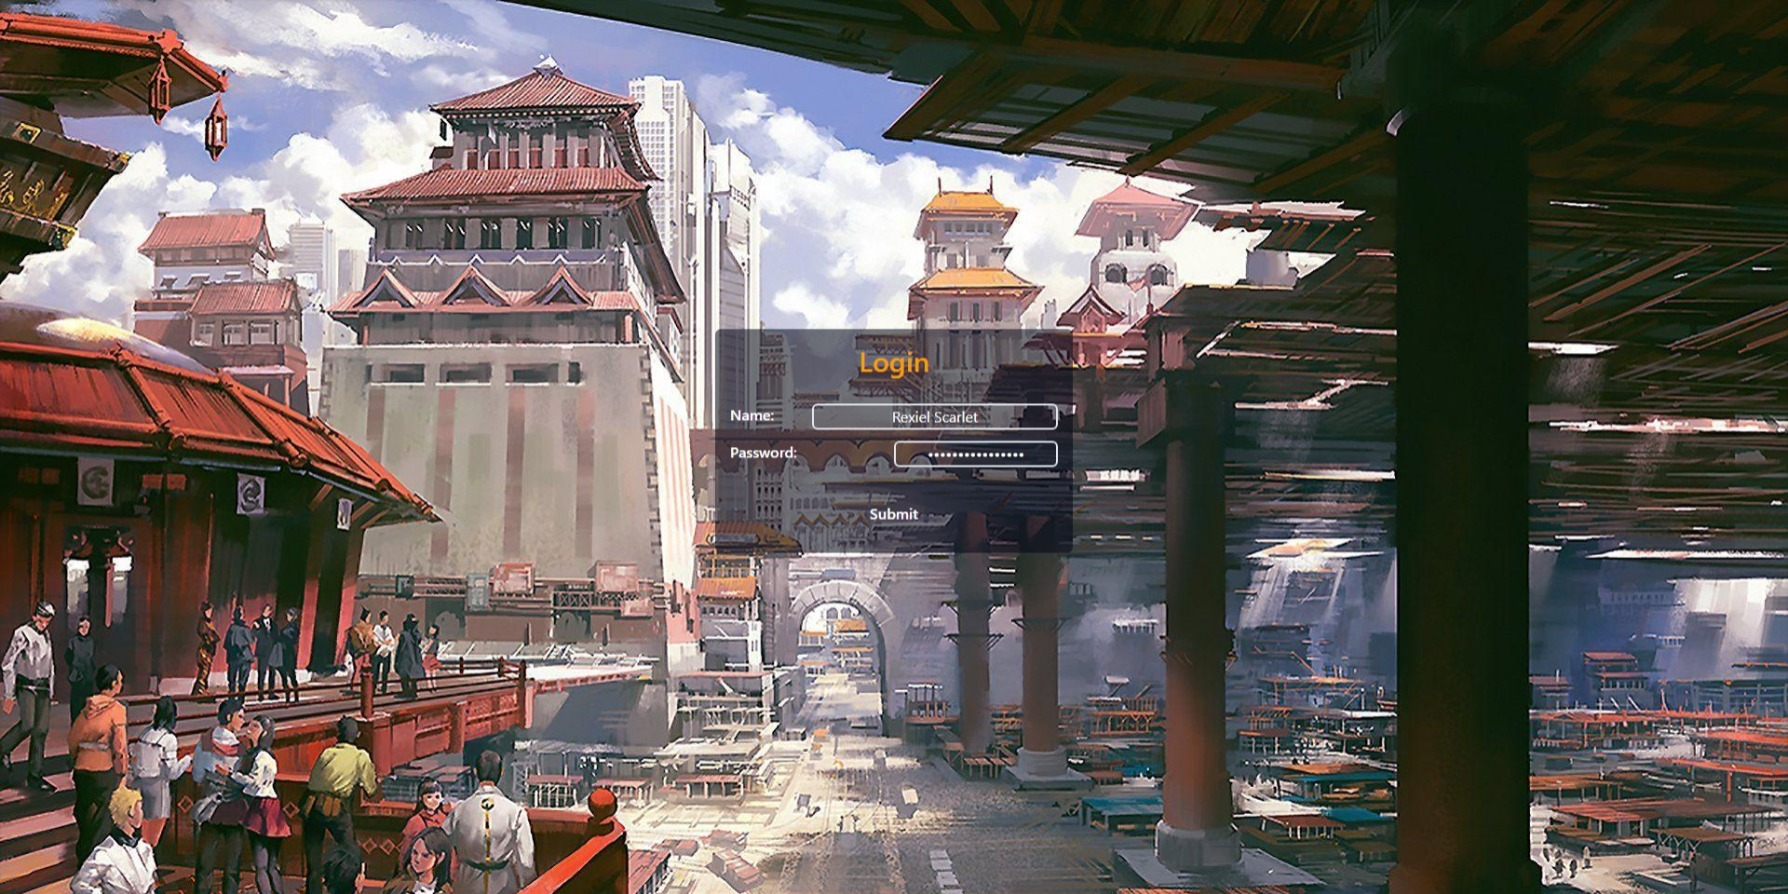
\includegraphics[width=1\textwidth]{./Assets/p1601.jpeg}
	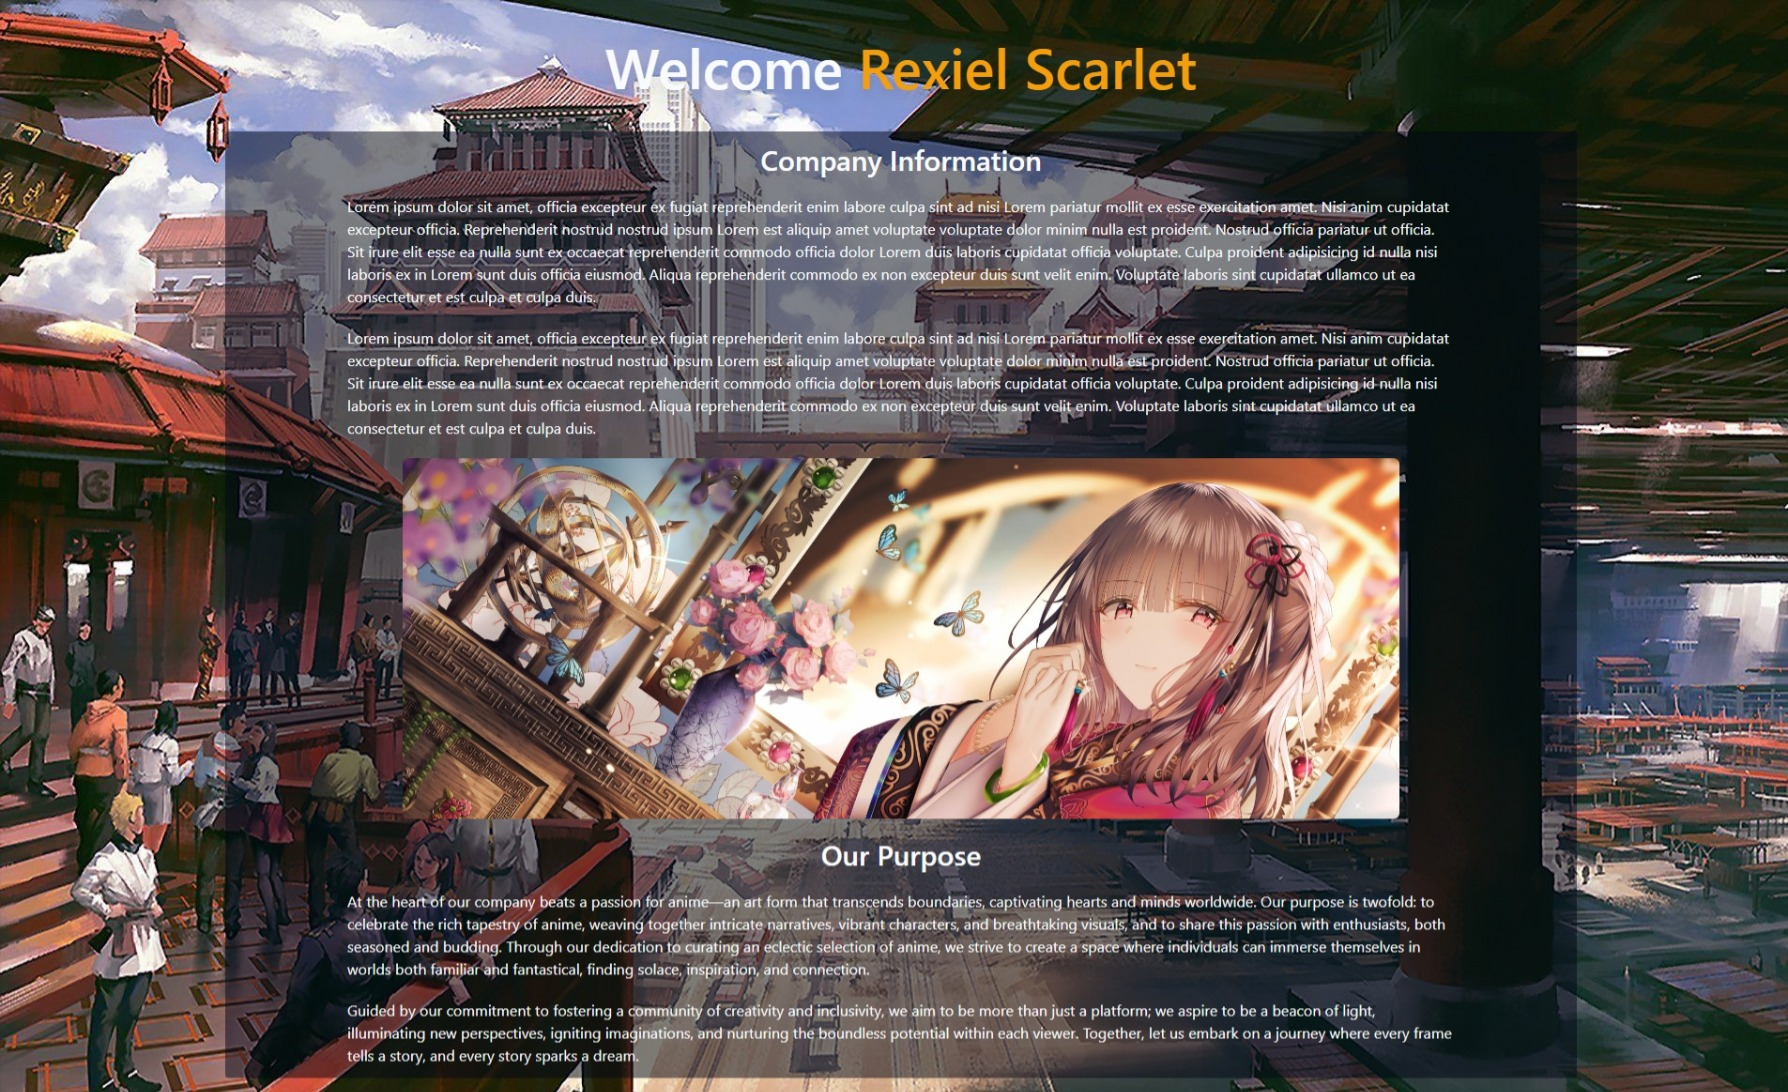
\includegraphics[width=1\textwidth]{./Assets/p1602.jpeg}
\end{figure}
\newpage

\section{Registration Form}
\subsection{Aim}
\begin{itemize}
  \item Write a Javascript program to validate a form with the following fields
  \item Name, Email, Country code (text)
  \item Zip Code (Drop Down)
\end{itemize}

\subsection{Code}
\inputminted[frame=lines, breaklines, breakanywhere, numberblanklines=false]{html}{./prog_17/index.html}

\subsection{Output}
\begin{figure}[h!]
	\centering
	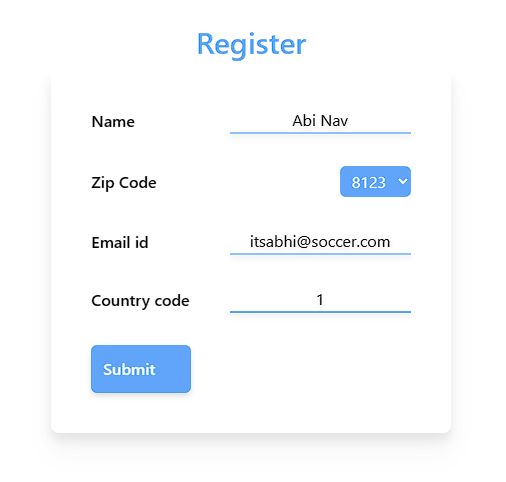
\includegraphics[width=0.7\textwidth]{./Assets/p17.png}
\end{figure}
\newpage

\section{Hiding with JQuery}
\subsection{Aim}
\begin{itemize}
  \item Use the JQuery library to hide elements using the different kinds of selectors
  \item make a drop down list which can be used to select what element is hidden
\end{itemize}

\subsection{Code}
\inputminted[frame=lines, breaklines, breakanywhere, numberblanklines=false]{html}{./prog_18/index.html}

\subsection{Output}
\begin{figure}[h!]
	\centering
	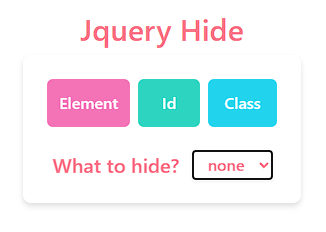
\includegraphics[width=0.4\textwidth]{./Assets/p1801.png}
	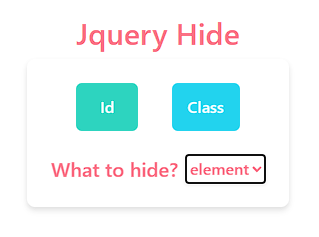
\includegraphics[width=0.4\textwidth]{./Assets/p1802.png}
\end{figure}
\begin{figure}[h!]
	\centering
	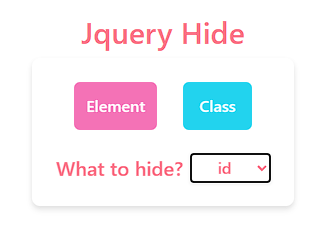
\includegraphics[width=0.4\textwidth]{./Assets/p1803.png}
	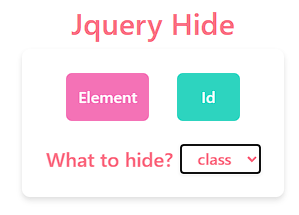
\includegraphics[width=0.4\textwidth]{./Assets/p1804.png}
\end{figure}
\newpage

\section{Online Railway Booking}
\subsection{Aim}
\begin{itemize}
  \item Design a website for booking online railway tickets having the following fields:
  \item Name, email, gender (radio)
  \item Date of Journey 
  \item Destination (dropdown)
\end{itemize}

\subsection{Code}
\inputminted[frame=lines, breaklines, breakanywhere, numberblanklines=false]{html}{./prog_19/index.html}

\newpage
\subsection{Output}
\begin{figure}[h!]
	\centering
	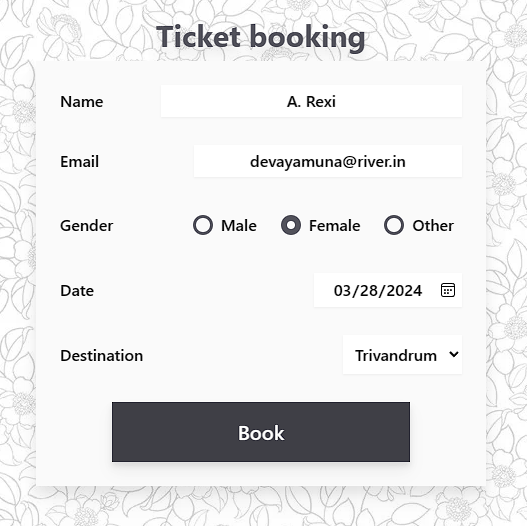
\includegraphics[width=0.7\textwidth]{./Assets/p19.png}
\end{figure}
\newpage

\section{AJAX}
\subsection{Aim}
\begin{itemize}
  \item Write a JavaScript program utilizing AJAX technology
\end{itemize}

\subsection{Code}
\inputminted[frame=lines, breaklines, breakanywhere, numberblanklines=false]{html}{./prog_20/index.html}

\subsection{Output}
\begin{figure}[h!]
	\centering
	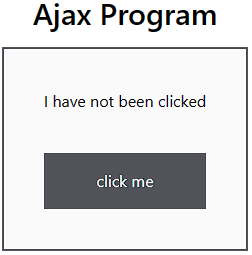
\includegraphics[width=0.25\textwidth]{./Assets/p2001.png}
	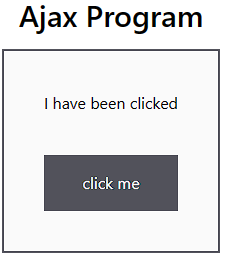
\includegraphics[width=0.25\textwidth]{./Assets/p2002.png}
\end{figure}
\newpage

\section{Customer Details}
\subsection{Aim}
\begin{itemize}
  \item Use php to display details from a form in tabular manner in a new page. The form contains the following fields
  \item customer number, name, place
  \item email ID \& phone number
\end{itemize}

\subsection{Code}
index.html
\inputminted[frame=lines, breaklines, breakanywhere, numberblanklines=false]{html}{./prog_21/index.html}
table.php
\inputminted[frame=lines, breaklines, breakanywhere, numberblanklines=false]{php}{./prog_21/table.php}

\subsection{Output}
\begin{figure}[h!]
	\centering
	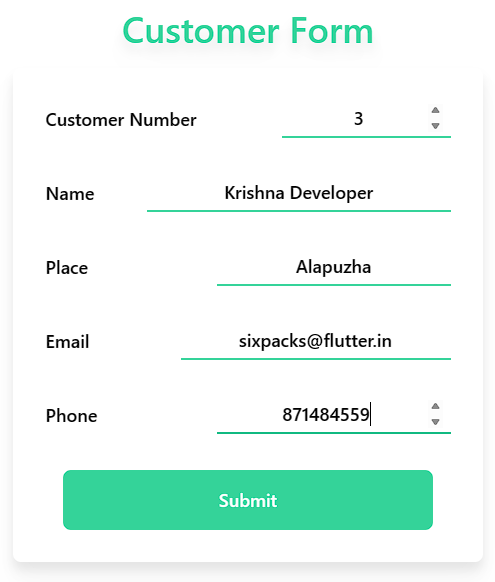
\includegraphics[width=0.5\textwidth]{./Assets/p2101.png}
	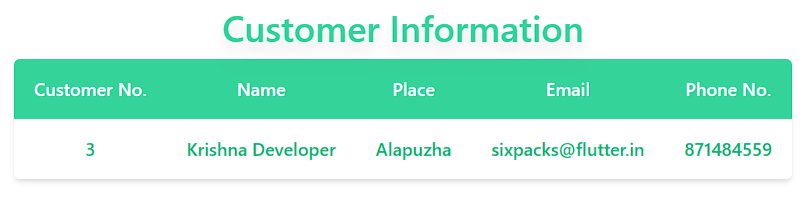
\includegraphics[width=1\textwidth]{./Assets/p2102.png}
\end{figure}
\newpage

\section{Number of Visitors}
\subsection{Aim}
\begin{itemize}
  \item Write a Php program to count the number of visitors
\end{itemize}

\subsection{Code}
index.php
\inputminted[frame=lines, breaklines, breakanywhere, numberblanklines=false]{php}{./prog_22/index.php}

\subsection{Output}
\begin{figure}[h!]
	\centering
	
\includegraphics[width=0.5\textwidth]{./Assets/p22.png}
\end{figure}
\newpage

\section{KSEB Login Page}
\subsection{Aim}
\begin{itemize}
  \item Write a Php program to login and view the Consumer Bill
\end{itemize}

\subsection{Code}
index.html
\inputminted[frame=lines, breaklines, breakanywhere, numberblanklines=false]{html}{./prog_23/index.html}
login.php
\inputminted[frame=lines, breaklines, breakanywhere, numberblanklines=false]{php}{./prog_23/login.php}

\subsection{Output}
\begin{figure}[h!]
	\centering
	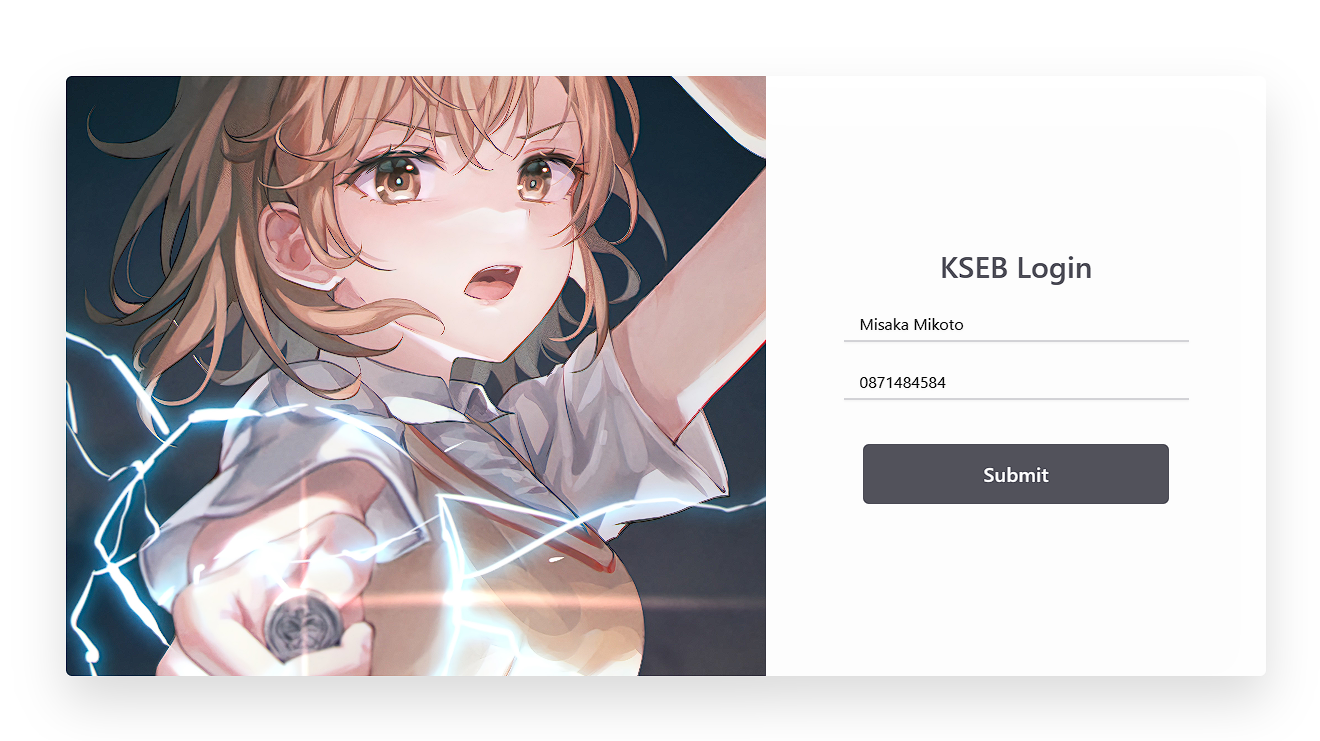
\includegraphics[width=1\textwidth]{./Assets/p2301.png}
	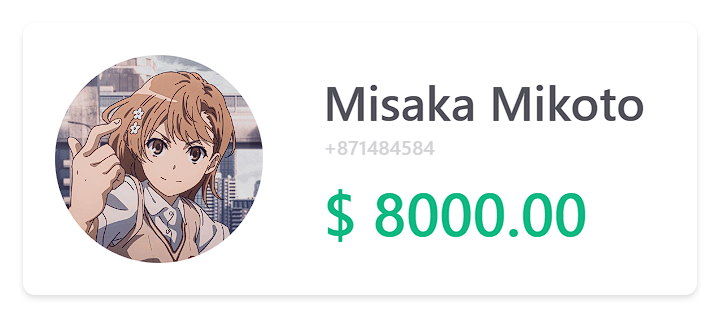
\includegraphics[width=0.5\textwidth]{./Assets/p2302.png}
	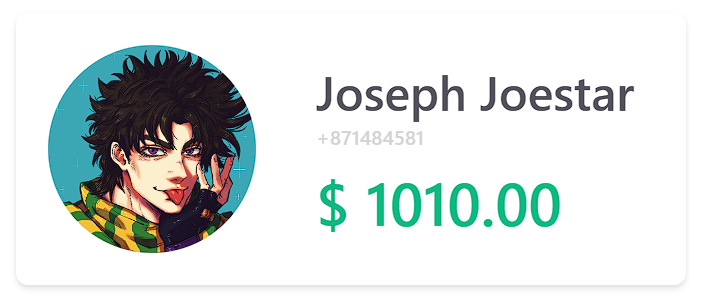
\includegraphics[width=0.5\textwidth]{./Assets/p2303.png}
\end{figure}
\newpage

\section{Online Applicaiton Form}
\subsection{Aim}
\begin{itemize}
  \item Write a Php program to display the details from an html form
\end{itemize}

\subsection{Code}
index.html
\inputminted[frame=lines, breaklines, breakanywhere, numberblanklines=false]{html}{./prog_24/index.html}
display.php
\inputminted[frame=lines, breaklines, breakanywhere, numberblanklines=false]{php}{./prog_24/display.php}

\subsection{Output}
\begin{figure}[h!]
	\centering
	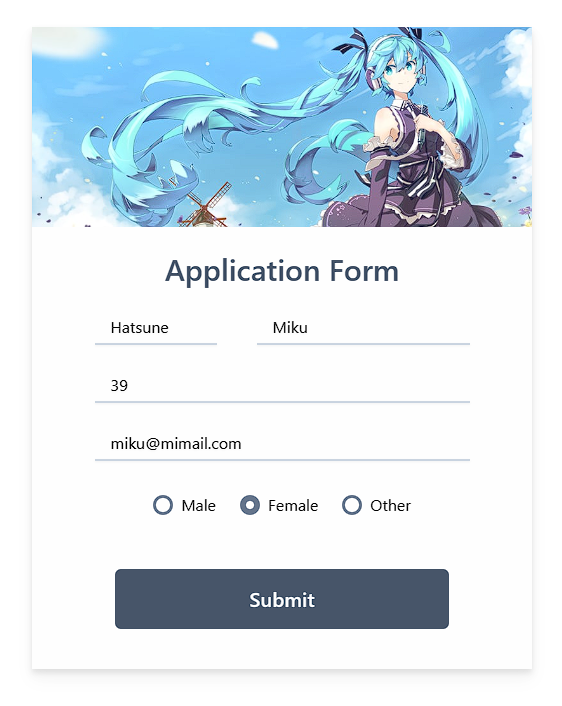
\includegraphics[width=0.5\textwidth]{./Assets/p2401.png}
	
\includegraphics[width=0.8\textwidth]{./Assets/p2402.png}
\end{figure}
\newpage

\section{Current Date Time Cookie}
\subsection{Aim}
\begin{itemize}
  \item Write a PHP program to store the current date and time in a cookie and display the last visited on date-time upon reopening the page
\end{itemize}

\subsection{Code}
\inputminted[frame=lines, breaklines, breakanywhere, numberblanklines=false]{php}{./prog_25/index.php}

\subsection{Output}
\begin{figure}[h!]
	\centering
	\includegraphics[width=0.8\textwidth]{./Assets/p25.png}
\end{figure}
\newpage
\section{Update Student Phone Number}
\subsection{Aim}
\begin{itemize}
  \item Write a PHP program to login with register no. and update the phone number
\end{itemize}

\subsection{Code}
index.html
\inputminted[frame=lines, breaklines, breakanywhere, numberblanklines=false]{html}{./prog_26/index.html}
update.php
\inputminted[frame=lines, breaklines, breakanywhere, numberblanklines=false]{php}{./prog_26/update.php}

\subsection{Output}
\begin{figure}[h!]
  \centering
  \caption{Submission without entering new phone number}
  \includegraphics[width=0.4\textwidth]{./Assets/p2601.png}
  \includegraphics[width=0.4\textwidth]{./Assets/p2602.png}
\end{figure}

\newpage
\begin{figure}[h!]
  \centering
  \caption{Submission with new phone number}
  \includegraphics[width=0.4\textwidth]{./Assets/p2603.png}
  \includegraphics[width=0.4\textwidth]{./Assets/p2604.png}
\end{figure}
\newpage
\section{Delete Student Entry}
\subsection{Aim}
\begin{itemize}
  \item Write a program to login as Admin and delete the details of a student from the university database
\end{itemize}

\subsection{Code}
index.html
\inputminted[frame=lines, breaklines, breakanywhere, numberblanklines=false]{html}{./prog_27/index.html}
login.php
\inputminted[frame=lines, breaklines, breakanywhere, numberblanklines=false]{php}{./prog_27/login.php}

\subsection{Output}
\begin{figure}[h!]
	\centering
  \caption{Correct Password and Valid Entry}
	\includegraphics[width=0.5\textwidth]{./Assets/p2701.png}
	\includegraphics[width=0.5\textwidth]{./Assets/p2702.png}
	\includegraphics[width=0.6\textwidth]{./Assets/p2703.png}
\end{figure}
\begin{figure}[h!]
	\centering
  \caption{Invalid Entry}
	\includegraphics[width=0.5\textwidth]{./Assets/p2704.png}
	\includegraphics[width=0.6\textwidth]{./Assets/p2705.png}
\end{figure}
\newpage
\begin{figure}[h!]
	\centering
  \caption{Wrong Password}
	\includegraphics[width=0.5\textwidth]{./Assets/p2706.png}
	\includegraphics[width=0.6\textwidth]{./Assets/p2707.png}
\end{figure}
\begin{figure}[h!]
	\centering
  \caption{Dataset}
	\includegraphics[width=0.6\textwidth]{./Assets/p2708.png}
\end{figure}
\newpage

\section{Session}
\subsection{Aim}
\begin{itemize}
  \item Write a PHP program to create, update, and delete a session
\end{itemize}

\subsection{Code}
index.php
\inputminted[frame=lines, breaklines, breakanywhere, numberblanklines=false]{html}{./prog_28/index.php}
create.php
\inputminted[frame=lines, breaklines, breakanywhere, numberblanklines=false]{html}{./prog_28/create.php}
destroy.php
\inputminted[frame=lines, breaklines, breakanywhere, numberblanklines=false]{html}{./prog_28/destroy.php}

\subsection{Output}
\begin{figure}[h!]
	\centering
  \caption{Session Creation}
	\includegraphics[width=0.4\textwidth]{./Assets/p2801.png}
	\includegraphics[width=0.4\textwidth]{./Assets/p2802.png}
\end{figure}
\begin{figure}[h!]
	\centering
  \caption{Session Updation}
	\includegraphics[width=0.5\textwidth]{./Assets/p2803.png}
	\includegraphics[width=0.5\textwidth]{./Assets/p2804.png}
\end{figure}

\newpage
\begin{figure}[h!]
	\centering
  \caption{Session Deletion}
	\includegraphics[width=0.5\textwidth]{./Assets/p2805.png}
	\includegraphics[width=0.5\textwidth]{./Assets/p2806.png}
	\includegraphics[width=0.5\textwidth]{./Assets/p2807.png}
\end{figure}
\newpage

\end{document}
